% !TEX TS-program = pdflatex
\documentclass[11pt,div=14]{scrartcl}

%Titel und Author
\newcommand\myTitle{Informationen zum Einrichten der Example-Umgebung}
\newcommand\myAuthor{Benjamin Dinkelmeyer, Andreas Lanzl und Sonnia Tsague}

%IKRSimlibSource
\newcommand\mySimLibSource{IKR-Homepage}
% Schrifteneinbindung in Abhängigkeit von der Engine
\usepackage{ifluatex}
\ifluatex
	\usepackage{fontspec}
	\setmainfont{TimesNewRoman}
\else
	\usepackage[utf8]{inputenc}
	\usepackage[T1]{fontenc}
	\usepackage{tgtermes}
\fi



\usepackage{pgfplots} 
\usepackage{subfigure}
\usepackage{listings}
\usepackage{color} 
% Hyperref und biblatex
\usepackage[colorlinks, linkcolor=black, citecolor=black, filecolor=black, urlcolor=black]{hyperref}
%\usepackage[backend=biber,style=numeric,citestyle=numeric-comp,hyperref=true,backref=true,block=none,maxcitenames=3,maxbibnames=100]{biblatex}
\usepackage{booktabs}
\usepackage[style=numeric] {biblatex}



% Abstände vor und nach Überschriften
\usepackage{titlesec}
\titlespacing*{\section}{0pt}{12pt}{6pt}
\titlespacing*{\subsection}{0pt}{12pt}{6pt}

% Abstände vor Absätzen
\usepackage{parskip}
\setlength{\parindent}{0pt}
\setlength{\parskip}{6pt}

%Weitere Pakete
\usepackage[singlespacing]{setspace}
\usepackage{caption}
%\usepackage{minted}
\usepackage{array} 
\usepackage{ amssymb,amsmath }
\usepackage[ngerman]{babel}
\usepackage{csquotes}
\usepackage{graphicx}
%\usepackage[tmargin=1in,bmargin=2cm,lmargin=1in,rmargin=1in]{geometry}
\usepackage{wrapfig}

% Schrifteinstellungen
\addtokomafont{disposition}{\rmfamily\normalfont}
\addtokomafont{section}{\rmfamily\bfseries}
\addtokomafont{subsection}{\rmfamily\bfseries\Large}

% Titel

\title{\LARGE \vspace*{-30pt} Technische Hochschule Ingolstadt \\ \vspace{10pt} Projekt \\ TCP \\ \vspace{6pt}{\Large Wintersemester 16/17 \vspace{40pt} \\ Projektdoku\vspace{10pt} \\ \myTitle \vspace{10pt} \\ von \\ \vspace{6pt}  \myAuthor} \vspace*{-36pt}}
\author{}
\date{}

%Satzspiegel
\KOMAoptions{DIV=14}

\usetikzlibrary{positioning}
\usepackage{hyperref}
\begin{document}
\maketitle% this prints the handout title, author, and date
\tableofcontents 

\definecolor{lightred}{rgb}{1,0.5,0.5} 
\lstset{ 
language=bash, 
basicstyle=\ttfamily, 
numbersep=5pt, 
backgroundcolor=\color{lightred}, 
showspaces=false, 
frame=single, 
tabsize=2, 
breaklines=true, 
prebreak={\textbackslash} 
} 

\section{Allgemeine Infos}
\label{Allgemeine Infos}
In diesem Dokument wird beschrieben, wie die Umgebung zu installieren ist (siehe \ref{Installation der Umgebung}), zeigt wie man eine Simulation erstellt (\ref{Simulation}) und listet einige ausgeführte Beispiele auf (\ref{Ausführungsbeispiele}), die mit der IKR-SimLib erstellt worden sind. Zudem ist eine \nameref{Befehlskette} aufgelistet, die dem Benutzer die Ausführung erleichtern soll. Abschießend sind noch eine Hand voll 'known Bugs' in \ref{Known issues} gelistet.
Mit der IKR-Simlib (zu finden unter \url{www.ikr.uni-stuttgart.de/IKRSimLib}) kann Netzwerkverkehr simuliert und grafisch dargestellt werden. Die Datei \textit{TutorialSimLib} liefert noch viele weitere Informationen. Zudem sind dort auch einige Ausführungsbeispiele zu finden.\\
\textbf{Achtung: Für die Ausführung des Simulationen ist ein Debian-Linux-System zu verwenden. Zuzüglich werden Adminrechte benötigt}


\section{Installation der Umgebung}
\label{Installation der Umgebung}
Über das Installationsskript \textit{QemuSimlibEnvInstall.sh} (im Git-Repository  im ZIP-File \textit{SimLibEnvironment}zu finden) ist die Installation der Umgebung ein Kinderspiel. \marginpar{Danke Andi :)}
\begin{enumerate}
\item Download des ZIP-Files
\item Die ZIP-Datei auf einem Ubuntu/Debian System entpacken

\item In einer Shell zum Verzeichnis springen (z.B. 
\colorbox{lightred}{\lstinline$cd ~/Schreibtisch/SimLibEnv$})


\item Das Skript ausführen: \colorbox{lightred}{\lstinline$./create-simlib-qemu-simulation.sh <Beliebiger Ordnername>$} \\ z.B. kann der Befehl so lauten: \colorbox{lightred}{\lstinline$./create-simlib-qemu-simulation.sh myFancyIKRFolder$}\\ Das Skript lädt nun alle erforderlichen IKR-SimLib-Dateien und konfiguriert diese und erzeugt noch einige nützliche Skripte. Die SimLib-Installationsdateien, welche für den Anwender eher unrelevant sind, liegen im Ordner \textit{install}. Die wichtigen Dateien sind in dem Ordner zu finden, dessen Namen man bei der Ausführung des Skripts mitgegeben hat (hier: \textit{myFancyIKRFolder}). Der Inhalt des Ordners ist in Abbildung \ref{fig:Ordnerinhalt} zu sehen. 

\begin{figure}[h!]
\centering
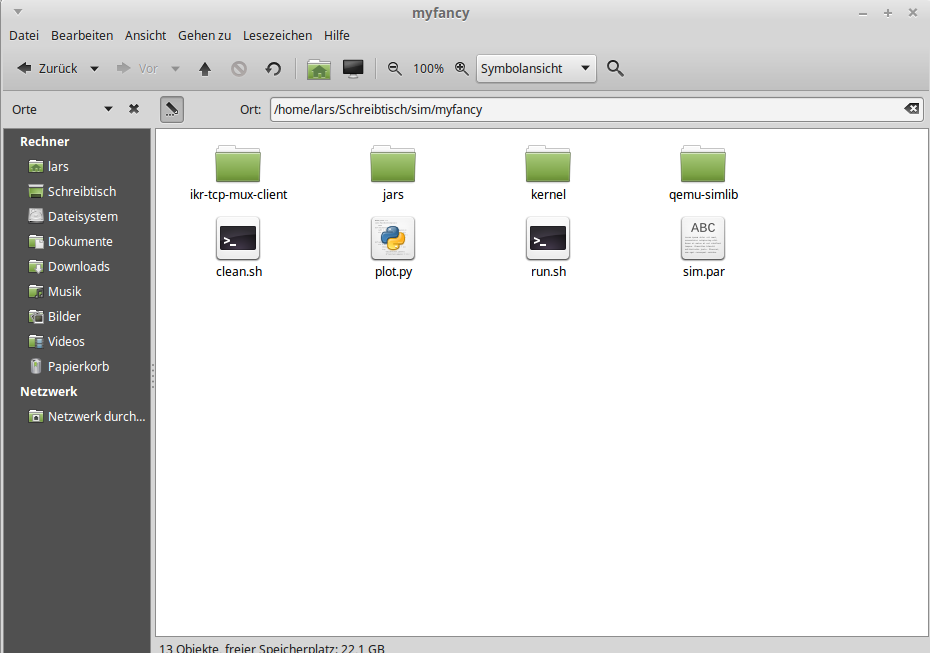
\includegraphics[scale=0.75]{bilder/vorSimulation.png}%
\caption{Der Ordnerinhalt nach Ausführung des Installers}%
\label{fig:Ordnerinhalt}%
\end{figure}

\item Wenn es keine Fehler gab, kann fröhlich drauf los simuliert werden \#smiley - hierfür siehe nächstes Kapitel \nameref{Simulation}
\end{enumerate}

\section{Simulation}
\label{Simulation}
In der Abbildung \ref{fig:Ordnerinhalt} sind einige wichtigen Dateien erkennbar:
\begin{description}
\item[sim.par] Ist die Parameterdatei, die die Simulation konfiguriert. Das heißt, diese Datei wird verändert um andere Ergebnisse zu erhalten. Über \colorbox{lightred}{\lstinline$vim sim.par$} kann man sich die Konfiguration ansehen. Alternative zum vim ist natürlich ein grafischer Texteditor ihrer Wahl.
\item[run.sh] Ist ein Skript, das die Simulation startet
\item[plot.py] Ist ein Skript, das die Ergebnisse grafisch (via Python) darstellt.
\item[view.sh] Ist ein Skript, das die Ergebnisse grafisch (via Xmgrace; heißt: nicht so schön) darstellt.
\end{description}

Um die \textbf{erste Simulation} zu starten wechselt man über 
\colorbox{lightred}{\lstinline$cd <OrdnerName>$} in den Ordner mit den wichtigen Skripten. Hier führt man den Befehl \colorbox{lightred}{\lstinline$./run.sh$} aus und lehnt sich zurück. Es wird nun anhand der sim.par die Kommunikation simuliert. Das Ergebnis ist in Abbildung \ref{fig:OrdnerinhaltNachrunsh} zu sehen.

\begin{figure}[h!]
\centering
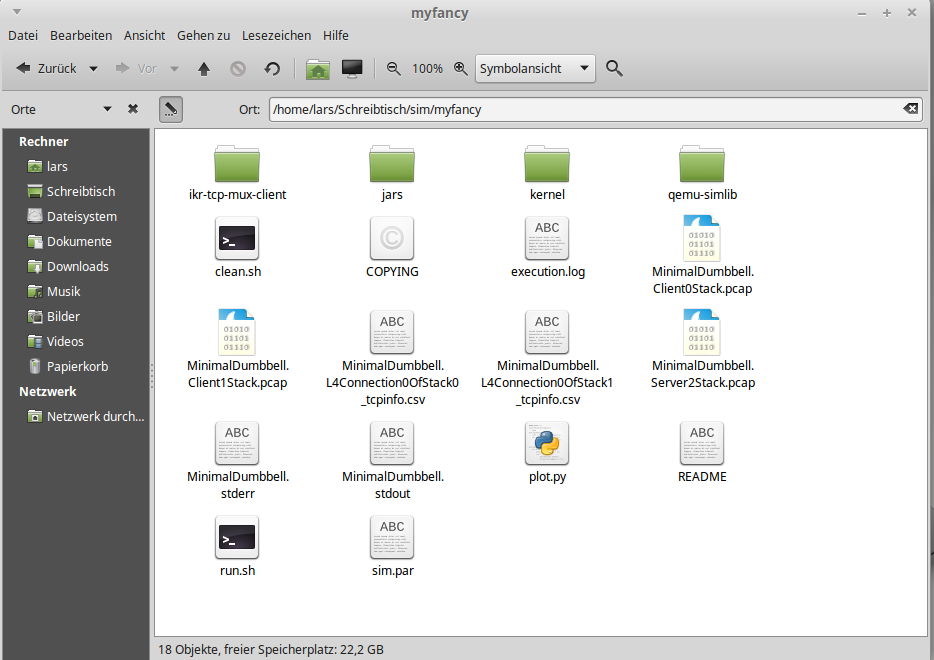
\includegraphics[scale=0.75]{bilder/nachSimulation.png}%
\caption{Der Ordnerinhalt nach Ausführung von run.sh}%
\label{fig:OrdnerinhaltNachrunsh}%
\end{figure}

Man erkennt, dass einige neue Dateien hinzugekommen sind.
Die Wichtigsten sind im Folgenden erklärt: 
\begin{description}
\item[*.pcap] sind die Dateien, die den Netzwerkverkehr im Wireshark nachvollziehbar machen. Die Files können im Wireshark geöffnet werden. Hierzu den in die Konsole \textit{wireshark} eingeben und eines der .pcap-Files öffnen.

\item[MinimalDumbbel.L4Conection0OfStack\textbf{*}\_tcpinfo.csv] Enthält die Simulationsergebnisse in tabellarischer Form. Dieses kann ebenfalls über z.B.  \colorbox{lightred}{\lstinline$vim MinimalDumbbel.L4Conection0OfStack0_tcpinfo.csv$} angezeigt werden. Der Stern steht hier für den jeweiligen Client (0 bis n-1). 

\item[MinimalDumbbell.stdout] Logfile für die Standardausgabe
\item[MinimalDumbbell.stderr] Logfile für die Standardfehlerausgabe

Abschließend kann man über \\
\colorbox{lightred}{\lstinline$python plot.py MinimalDumbbell.L4Connection0OfStack0_tcpinfo.csv$} (python Darstellung)
\\oder\\
\colorbox{lightred}{\lstinline$./view.sh MinimalDumbbell.L4Connection0OfStack0_tcpinfo.csv$} (xmgrace Darstellung)
\end{description}

Das \textit{plot.py}-Python-Skript ist so implementiert, dass nur das Conjestion Window angezeigt wird. Hierfür wird die .csv-Datei mit dem einfachen plot.py aufgerufen.

%\marginpar{OBACHT: Fehlerquelle}
Wenn man im \textit{sim.par}-File die letzte Zeile (MinimalDumbbell.L4Connection*.LoggedTcpInfoValues...) nicht kommentiert, werden mehr Messwerte (Treshhold usw.) festgehalten und bei der graphischen Visualisierung farblich getrennt dargestellt.
% \textbf{MÜSSEN} die *.csv-Dateien mit dem \textit{python-L4Connection}-Skript aufgerufen werden 

Um mehrere Ergebnisse gleichzeitig anzuzeigen, kann man das eines der beiden python-Skripte mit dem *-Operator aufrufen: z.B. \colorbox{lightred}{\lstinline$python plot.py MinimalDumbbell.L4Connection0OfStack*_tcpinfo.csv$}. Dies macht natürlich nur Sinn, wenn mehrere Clients oder mehrere Server in der Simulation beteiligt waren.

Für die nächste Simulation muss man 'nur' die Datei \textit{sim.par} anpassen, run.sh und das Pythonskript oder das Shellskript für die grafische Visualisierung ausführen.

Sollte bei einem Plot auffallen, dass der SlowStart einen extrem hohen Wert erreicht hat, so sind alle weiteren Ergebnisse sehr klein und nahe der x-Achse angesiedelt. Um dies zu umgehen, kann über \textbf{scale} eine maximale Höhe für den Plot angegeben werden.\\ z.B. \colorbox{lightred}{\lstinline$python plot.py MinimalDumbbell.L4Connection0OfStack*_tcpinfo.csv scale 1000$}.

Im Tutorial \textit{$tutorial_SimuLib-IRK$} sind bereits einige Beispiele ausgeführt und die jeweiligen sim.par-Einstellungen hinterlegt. Diese kann kopiert werden, um das selbe Ergebnis zu simulieren. Die fertigen sim.par Dateien liegen im Ordner \textit{param-templates}.
\section{Ausführungsbeispiele}
\label{Ausführungsbeispiele}
Eine schnelle sichtbare Änderung erhält man, wenn man für \textit{DumbbellModel.DefaultCongestionControl = reno} konfiguriert.
In Abbildung \ref{fig:Transmissionrate} wurde die Transmissionrate jeweils einmal auf 15 $\frac{Mbit}{s}$ bzw. 25 $\frac{Mbit}{s}$  gedrosselt/erhöht. Wie zu erkennen ist, ist die ConjuestionWindow bei einer höheren Transmissionrate erhöht. 

In Abbildung \ref{fig:3C1S} wurden drei Clients und ein Server in der Standard sim.par konfiguriert. Man kann gut erkennen, dass zu jedem Zeitpunkt die Summe aller ConjestionWindows ungefähr gleich bleibt. 


\section{Befehlskette}
\label{Befehlskette}
Die Befehlskette ist in der Regel folgende:
\begin{description}
\item[sim.par editieren] \colorbox{lightred}{\lstinline$vim sim.par$}
\item[run.sh ausführen] \colorbox{lightred}{\lstinline$./run.sh$}
\item[Ergebnisse visualisieren] \colorbox{lightred}{\lstinline$python plot.py MinimalDumbbell.L4Connection0OfStack*_tcpinfo.csv$}
\item[Ergebnisse anzeigen] \colorbox{lightred}{\lstinline$vim MinimalDumbbell.L4Connection0OfStack0_tcpinfo.csv$}
\end{description}


\section{Known Issues (ohne Gewähr)}
\label{Known issues}
\begin{itemize}
\item In der Datei sim.par muss zwischen jedem '=' ein Leerzeichen sein, sonst kommt es zu Fehlern!
\end{itemize}



\begin{figure}
\centering
    \subfigure[TransmissionRate von 15 $\frac{Mbit}{s}$]{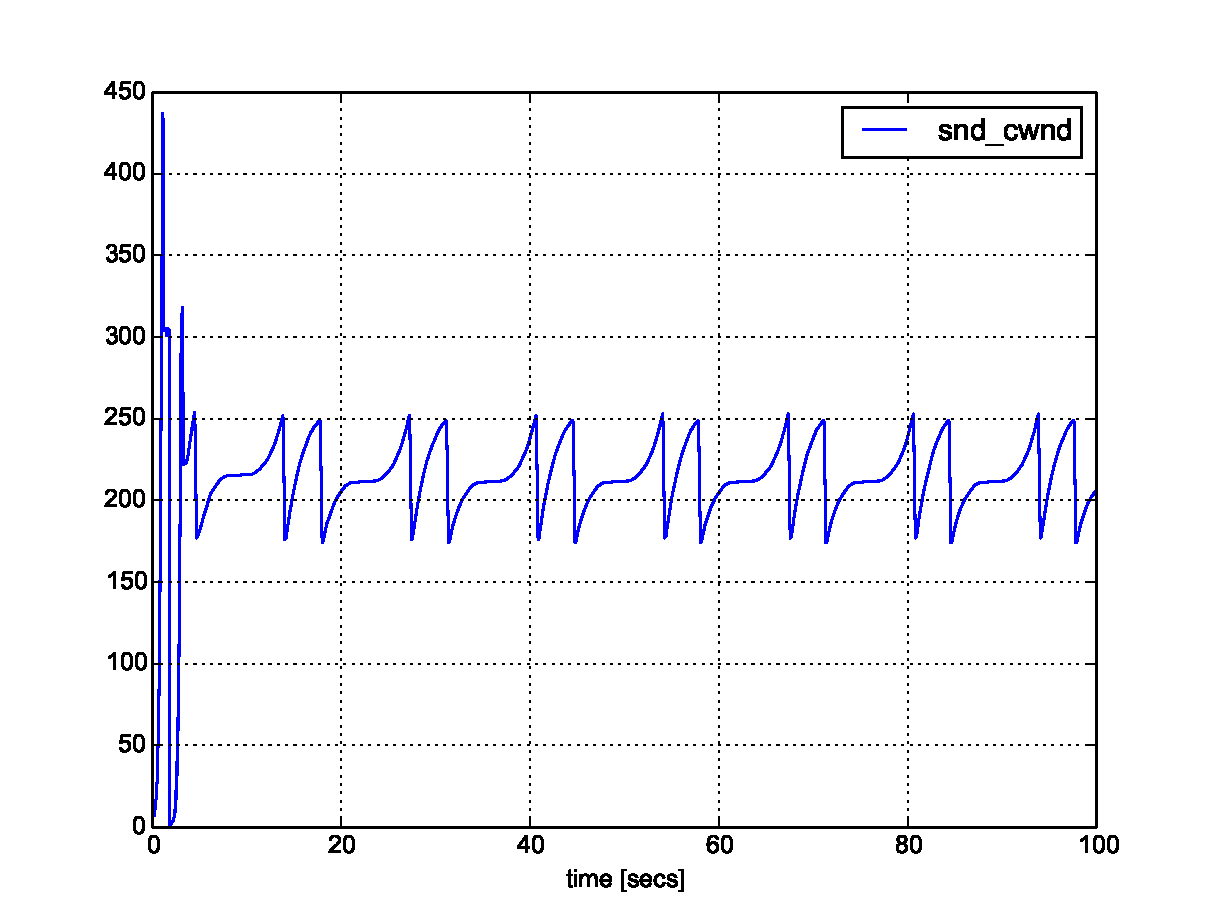
\includegraphics[width=0.45\textwidth]{bilder/ergebnis_-TrasnmissionRateInMbits-15-value-.pdf}} 
     \subfigure[TransmissionRate von 25 $\frac{Mbit}{s}$]{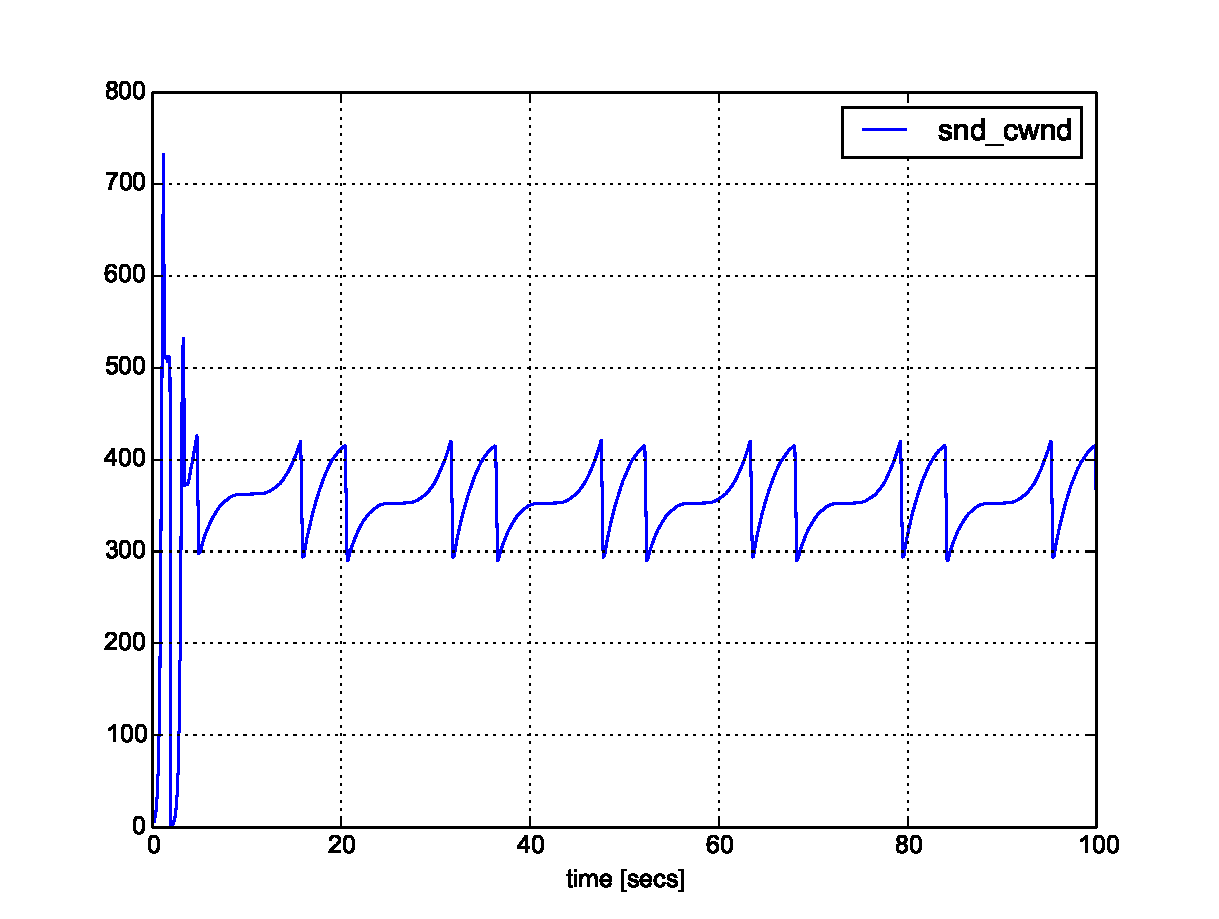
\includegraphics[width=0.45\textwidth]{bilder/ergebnis_-TrasnmissionRateInMbits-25-value-.pdf}} 
     \caption{Transmissionrate}
\label{fig:Transmissionrate} 
\end{figure}

\begin{figure}
\centering
    \subfigure[Verlauf der Simulation von \textbf{Client 1}]{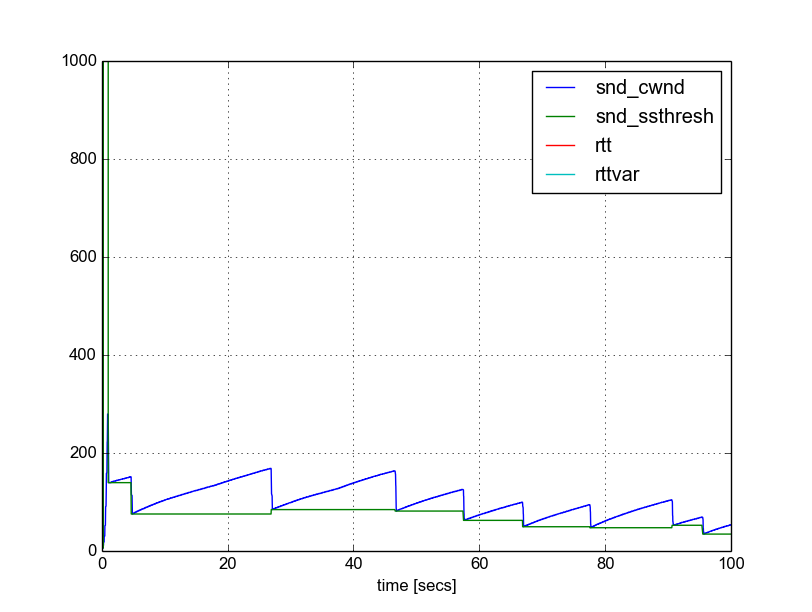
\includegraphics[width=0.7\textwidth]{bilder/3C1S_Client1.png}} 
     \subfigure[Verlauf der Simulation von \textbf{Client 2}]{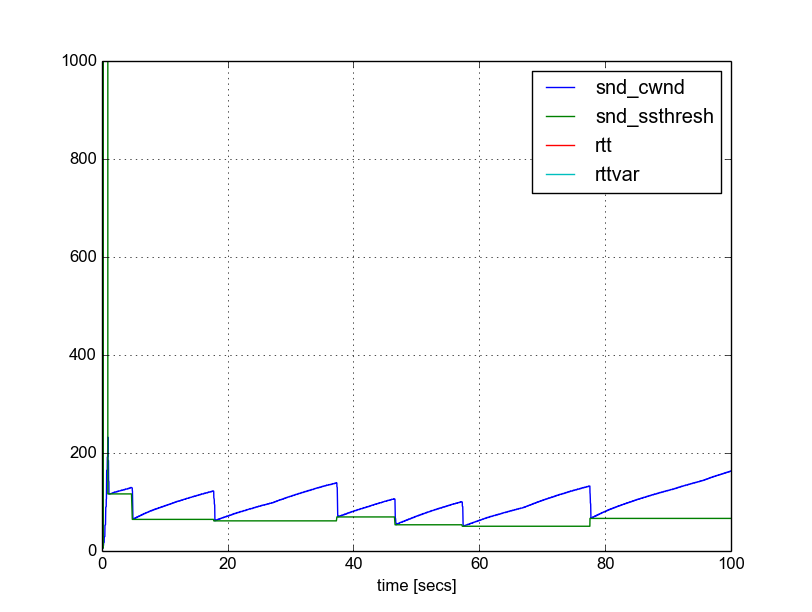
\includegraphics[width=0.7\textwidth]{bilder/3C1S_Client2.png}} \subfigure[Verlauf der Simulation von \textbf{Client 3}]{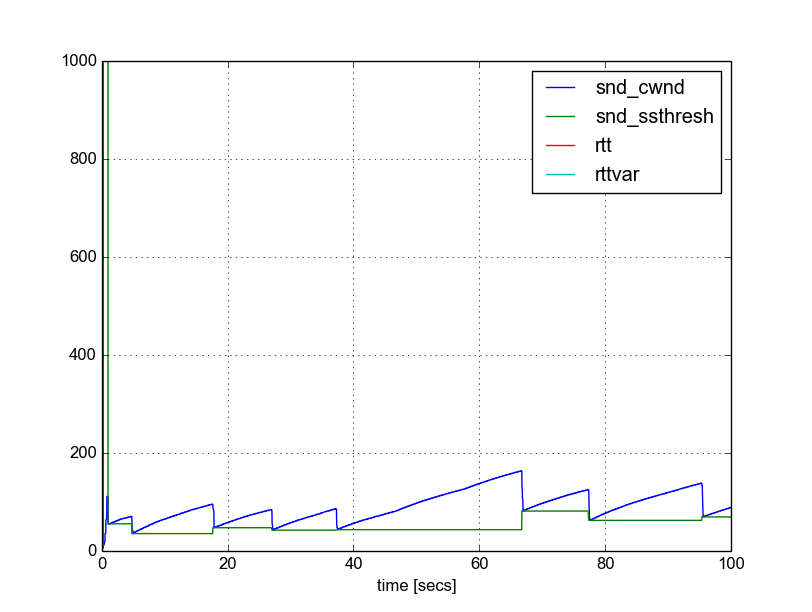
\includegraphics[width=0.7\textwidth]{bilder/3C1S_Client3.png}}  
\caption{3 Clients 1 Server}
\label{fig:3C1S} 
\end{figure}



\end{document}